\documentclass[13pt,compress,c]{beamer}
\usepackage[brazil]{babel}
\usepackage[latin1]{inputenc}
\usepackage{listings}
\usepackage{latexsym}
\usepackage{amssymb}
\usepackage{graphicx}
\usepackage{relsize}          % for \smaller etc.


%\bibliographystyle{plain}

\setbeamercolor{normal text}{bg=blue!4}

%\usetheme{default}

% tema com vermelho
%\usetheme{CambridgeUS}

% tema com amarelo
%\usetheme{AnnArbor}

% tema azul
\usetheme{Boadilla}

% tema azul, aulas de mc348 e mc448
%\usetheme{Madrid}

% tema mais branco
%\usetheme{umbc1} 

\title[Codifica��o por Apagamento no HDFS]{Estudo e Implementa��o de Mecanismos de Codifica��o por Apagamento no Sistema de Arquivos Distribu�do do Hadoop}

\author[Celina d' �. Samogin]{Celina d' �vila Samogin\\
  Instituto de Computa��o --- UNICAMP}

\begin{document}

\frame{

   \begin{center}
     \large{Proposta de Disserta��o de Mestrado}
    \end{center}

    \titlepage

    \begin{center}
     Orientadora: Profa. Dra. Islene Calciolari Garcia
    \end{center}

}


% \section{Agenda}

\AtBeginSection[]
{
  \begin{frame}
   \frametitle{Agenda}
   \tableofcontents[currentsection]
  \end{frame}
}


 \frame{\tableofcontents}

\AtBeginSection[]
{
  \begin{frame}
   \frametitle{Agenda}
   \tableofcontents[currentsection]
  \end{frame}
}

 \section{Introdu��o}

A codifica��o por apagamento (\emph{erasures codes}) introduz
redund�ncia em um sistema de transimiss�o ou armazenamento de dados de
maneira a permitir a detec��o e corre��o de erros. A codifica��o por
apagamento �, desde os anos 70, utilizada pela \emph{NASA's Deep Space
  Network} para receber sinais e dados de telemetria
(\emph{downlinks}) vindos de ve�culos espaciais (\emph{very distant
  spacecrafts}) e para enviar telecomandos (\emph{uplinks}) para
ve�culos espaciais \cite{Almeida:2007, STO:2010, TDD:2010}.

A t�cnica de codifica��o por apagamento pode ser combinada com a
distribui��o de dados entre v�rios dispositivos de armazenamento, o
que permite o aumento da largura de banda e a corre��o de
erros~\cite{Woitaszek:2007, Plank:1997}. Requisitos de confiabilidade
e de redu��o do tamanho do armazenamento podem ser observados em
sistemas que tratam de: \emph{digital fountain} (\emph{multicasting}
multim�dia confi�vel)\cite{Byers:1998}; \emph{Delay and Disruption
  Tolerant Networks}, redes de sensores e redes~\emph{peer-to-peer}
\cite{Rodrigues:2005, RTAD:2007, Houri:2009} e armazenamento de grande
volume de dados \cite{Kubiatowicz:2000, Weatherspoon:2002, Fan:2009},
como tamb�m o sistemas de arquivos distribu�do do Hadoop
(HDFS)~\cite{HDFS-503:2010}.

O HDFS, por padr�o, implementa alta disponibilidade dos dados via
replica��o simples dos blocos de dados. Esta abordagem acarreta um
alto custo de armazenamento para garantir que os dados estar�o sempre
dispon�veis. O objetivo do uso da codifica��o por apagamento no HDFS �
permitir que o espa�o de armazenamento possa ser reduzido sem
prejudicar a disponibilidade dos dados. Esfor�os iniciais nessa linha
foram feitos utilizando t�cnicas de RAID~\cite{HDFS-503:2010} e mais
recentemente do algoritmo Reed-Solomon~\cite{MR-1969:2010}.

Este trabalho pretende avan�ar esta linha de pesquisa a partir dos
seguintes passos:

\begin{itemize}
\item avalia��o de desempenho, ganhos, e custos de diferentes
  estrat�gias de codifica��o por apagamento;

\item implementa��o de otimiza��es ou extens�es para o c�digo que
  atualmente implementa Reed-Solomon, tentando melhorar,
  principalmente, a parte de distribui��o de blocos;

\item implementa��o de novos algoritmos (e.g., Tornado codes) e
  exten��o da interface atual para aceit�-los;

\item integra��o do c�digo atual com o HDFS.

\end{itemize}

O texto a seguir est� organizado da seguinte maneira: a Se��o 2
introduz os conceitos b�sicos da codifica��o por apagamento, a Se��o 3
comenta o \emph{framework} Hadoop e seu sistema de arquivos, a Se��o 4
apresenta os objetivos deste trabalho e a se��o 5 cita as atividades
propostas e o cronograma de execu��o.




 \section{Codifica��o por Apagamento}

A codifica��o de mensagens no emissor antes da transmiss�o e a
decodifica��o das mensagens (possivelmente danificadas) que chegam ao
receptor, possibilita reparar os efeitos de um canal f�sico com ru�dos
\cite{Shannon:1948} sem sobrecarregar a taxa de transmiss�o de
informa��o ou o \emph{overhead} de armazenamento \cite{Lin:1983}.

% A ideia b�sica da codifica��o �tima por apagamento � que o objeto
% original possa ser reconstru�do a partir de quaisquer $m$ �nicos
% fragmentos que s�o aproximadamente do mesmo tamanho do objeto original
% \cite{Weatherspoon:2002}. Para uma codifica��o quase �tima, s�o
% necess�rios $(1+e) \times m$ fragmentos, onde $e \geq 1$
% \cite{EC:2010}.

%Um dos principais par�metros de um c�digo para detec��o de erros � a
%probabilidade de detec��o de erro.

% A probabilidade de erro no canal determina a capacidade de
% transfer�ncia de informa��o no canal. Os modelos estudados por
% pesquisadores envolvem canais sim�tricos, assim�tricos e outros, com
% ou sem mem�ria~\cite{Weber:1985}. 

%Em canais bin�rios sim�tricos, assume-se que ambos os erros $0
%\rightarrow 1$ e $1 \rightarrow 0$ ocorrem com igual probabilidade.

Existem dois m�todos b�sicos para tratar erros em comunica��o e ambos
envolvem a codifica��o de mensagens. A diferen�a est� em como esses
c�digos s�o utilizados. Em um \emph{repeat request system}, os c�digos
s�o utilizados para detectar erros e se estes existirem, � feito um
pedido de retransmiss�o. Com \emph{forward error correction}, os
c�digos s�o usados para detectar e corrigir erros.

Na Figura~\ref{fig3:fec}, vemos um sistema que utiliza c�digo de
blocos. A fonte envia uma sequ�ncia de dados para o codificador. O
codificador divide esta sequ�ncia em $m$ blocos de $k$ \emph{bits}
cada chamados mensagens.  Uma mensagem � representada por uma
$k$-tupla bin�ria $u = u_1, u_2,\dots, u_k$. O codificador insere
\emph{bits} redundantes (ou de paridade) para cada mensagem $u$,
gerando uma sequ�ncia de sa�da de $n$ \emph{bits} chamada
\emph{codeword} ou palavra c�digo representada por uma $n$-tupla de
s�mbolos discretos $v = v_1, v_2, \dots, v_n$.  Os $n - k$ bits s�o os
bits redundantes que prov�m � codifica��o a capacidade de tratar os
ru�dos do canal.

\begin{figure}[htb]
  \setlength{\unitlength}{1cm}
  \begin{center}
  {\begin{picture}(12.5,6)(0,-3)
    \put(0,2){\framebox(3,1){Fonte}}
    \put(3,2.5){\vector(1,0){2}}
    \put(4,2.6){u}
    \put(5,2){\framebox(4,1){{Codificador (n,k)}}}
    \put(9,2.5){\line(1,0){2}}
    \put(10,2.6){v}
    \put(11,2.5){\vector(0,-1){2}}
    \put(9.5,-0.5){\framebox(3,1){Canal}}
    \put(6.8,-0.1){ru�dos}
    \put(8,-0){\vector(1,0){1.5}}
    \put(11,-0.5){\line(0,-1){2}}
    \put(11,-2.5){\vector(-1,0){2}}
    \put(10,-2.4){r}
    \put(0,-3){\framebox(3,1){Destino}}
    \put(5,-2.5){\vector(-1,0){2}}
    \put(4,-2.4){$\mathaccent 94 u$}
    \put(5,-3){\framebox(4,1){{Decodificador (n,k)}}}
   \end{picture}}
  \end{center}
  \caption{C�digos de bloco}
  \label{fig3:fec}
\end{figure}


% A gera��o de uma palavra c�digo depende apenas de um c�lculo alg�brico entre os $k$ bits, portanto, um codificador pode ser implementado como um circuito l�gico combinacional. O codificador executa o mapeamento: $T :  U \rightarrow V$ onde $U$ � um conjunto de palavras de dados de tamanho $k$ e $V$ � um conjunto de palavras c�digo de tamanho $n$ onde $n > k$. Cada uma das $2^k$ palavras de dados � mapeada para uma �nica palavra c�digo.

A taxa de codifica��o e o \emph{overhead} de armazenamento s�o
calculados a partir de $m$ blocos originais \cite{RTAD:2007,
  CMSC:2010}. S�o gerados $n$ s�mbolos pelo algoritmo de
codifica��o. $R = \frac{k}{n}$ � a taxa de codifica��o que pode ser
interpretada como o n�mero de bits de informa��o por palavra c�digo
transmitida e $O = \frac{1}{R}$ � o \emph{overhead} de armazenamento.

% Se $k \leq n$, mais bits redundantes podem ser adicionados, com aumento do tamanho da palavra c�digo, mantendo $R = \frac{k}{n}$ constante. Como escolher este n�mero $n - k$ de bits redundantes para obter transmiss�o confi�vel em cima de um canal com ru�dos � o problema principal do projeto do codificador. No destino, o decodificador extrai a sequ�ncia original de dados.

Outra m�trica utilizada � a redund�ncia que pode ser definida por
$\frac{(n - k)}{n}$. A alta redund�ncia aumenta a possibilidade de
todos os dados serem enviados em uma �nica transmiss�o. A desvantagem
da redund�ncia � que a adi��o de \emph{bits} pode exigir uma largura
de banda transmiss�o maior ou aumentar o atraso das mensagens (ou
ambos).

Segundo \cite{Woitaszek:2007}, para sistemas de armazenamento, a
codifica��o por apagamento baseada em opera��es simples, tais como XOR
RAID, s�o prefer�veis. Embora um mecanismo externo deva ser utilizado
para detectar erros, as opera��es de XOR podem ser realizadas
rapidamente e resultar em alto \emph{throughput} das opera��es de
codifica��o e decodifica��o.

Segundo \cite{Almeida:2007}, c�digos Reed-Solomon (RS) s�o
particularmente �teis para corre��o de erros em rajada (seq��ncia
s�mbolos consecutivos, nenhum desses recebidos corretamente, chamados
\emph{burst errors}). Tamb�m podem ser usados eficientemente em canais
em que o conjunto de s�mbolos de entrada � consideravelmente grande.

C�digos Tornado s�o uma classe de c�digos LDPC (Low Density Parity
Check) que utiliza grafos irregulares e que foi proposta por
M. Luby~\cite{Woitaszek:2007}. Segundo~\cite{Kubiatowicz:2000}, s�o
mais r�pidos para codificar e decodificar e necessitam de um pouco
mais de $m$ fragmentos para reconstruir a informa��o. Em
\cite{Byers:1998}, o autor comentou o tempo de decodifica��o para
c�digos RS e Tornado. C�digos Tornado usam equa��es com um n�mero
pequeno de vari�veis em contraste com c�digos RS.

Na tabela~\ref{tab1:comp}, alguns sistemas que utilizam com
codifica��o por apagamento foram comparados.


\begin{table}
\singlespacing

  \begin{center}
    \begin{tabular}{|p{2.5cm}||p{2cm}||p{2.7cm}||p{2.5cm}||p{3.5cm}|}
      \hline

Trabalho & Modelo & Objetivos & Codifica��o & M�tricas \\ \hline
Byers,1998 \cite{Byers:1998} & \emph{Digital Fountain} & Confiabilidade, Efici�ncia & Replica��o, c�digos Tornado e RS & tempo de codifica��o e decodifica��o de um bloco \emph{bandwidth}, perda de pacotes\\ \hline

Weatherspoon, 2002 \cite{Weatherspoon:2002} & Arquivador central, n�s & Disponibilidade & Replica��o, Codifica��o por Apagamento & tempo m�dio entre falhas, \emph{overhead} de armazenamento, tempo de verifica��o do bloco \\ \hline

Camargo, 2009 \cite{Camargo:2009} & OppStore & Confiabilidade, Disponibilidade & Replica��o  & \emph{bandwidth}, n�mero de mensagens trocadas \\ \hline

Fan, 2009 \cite{Fan:2009}& HDFS & Confiabilidade, Disponibilidade & Replica��o, RAID & atraso na codifica��o do bloco\\ \hline

Dabek, 2004 \cite{Dabek:2004} & DHT & Efici�ncia & Replica��o, Codifica��o por Apagamento & lat�ncia \\ \hline

Houri, 2009 \cite{Houri:2009} & \emph{Peer-to-peer} & Disponibilidade & Replica��o, Codifica��o por Apagamento & \emph{bandwidth} \\ \hline

Plank, 2009 \cite{Plank:2009} & $k$ discos de dados e $m$ discos de paridade & Efici�ncia & c�digos Tornado, RS e RAID & tempo de codifica��o de um grande arquivo de v�deo e tempo de decodifica��o de um \emph{drive} de dados\\ \hline
    \end{tabular}
\caption{Compara��o entre sistemas de codifica��o por apagamento}
\label{tab1:comp}
  \end{center}
\end{table}


\subsection*{Replica��o versus Codifica��o por Apagamento}

Para implementar redund�ncia de dados em sistemas, s�o utilizadas
v�rias t�cnicas: codifica��o por apagamento, replica��o, espelhamento,
\emph{Cyclic redundancy check} (CRC), \emph{bits} de paridade,
\emph{checksum} e assinatura digital. Mecanismos de
redund�ncia podem implementar um conjunto destas
t�cnicas~\cite{Fan:2009}.

A principal desvantagem da replica��o � que ela requer um grande
\emph{overhead} de armazenamento para pouco ganho em disponibilidade e
toler�ncia a falhas. Garantir que os dados permane�am dispon�veis
quando todos os $n$ dispositivos falham exige que, pelo menos, $n + 1$
c�pias existam~\cite{Woitaszek:2007}. Em \cite{Haeberlen:2005}, os
experimentos mostraram que o armazenamento no sistema Glacier
utilizando replica��o pura obteve um aumento de 11 vezes na quantidade
de dados armazenados para conseguir 0.999999\% de confiabilidade. Um
c�lculo da medida da quantidade de redund�ncia da replica��o pura e da
codifica��o chamada \emph{stretch factor} e a respectiva
disponibilidade pode ser encontrado em \cite{Bhagwan:2003}.

Os autores em \cite{Dabek:2004} afirmam que dados replicados permitem
leituras de baixa lat�ncia, porque h� muitas op��es para a sele��o de servidores,
enquanto que dados codificados reduzem o consumo de largura de banda para escritas,
em detrimento do aumento da lat�ncia de leituras.

Uma vantagem de codifica��o por apagamento seria um custo menor de
armazenamento se comparado a replica��o, no caso de grande volume de
dados. Outra vantagem com rela��o a replica��o foi comentada em
\cite{Weatherspoon:2002}: para um mesmo espa�o de armazenamento, o
tempo m�dio entre falhas (\emph{mean time to failure}) � maior.

Em \cite{Kubiatowicz:2000} e \cite{Weatherspoon:2002}, os pesquisadores concluem
que o uso de codifica��o por apagamento aumenta significativamente a disponibilidade de dados.

A Figura~\ref{fig4:srp} apresenta um sistema de arquivos distribu�dos armazenando um arquivo particionado em 8 blocos. O fator de replica��o � 4. Os clientes precisam que, para cada um dos 8 distintos blocos, uma das quatro c�pias esteja dispon�vel. A Figura~\ref{fig5:crs} apresenta o mesmo sistema que a Figura~\ref{fig4:srp}, mas utilizando c�digos RS. O arquivo est� particionado em 8 blocos e 32 blocos codificados foram gerados. Os clientes podem utilizar quaisquer 8 blocos para obter o arquivo inicial. A Figura~\ref{fig5:crs} tamb�m se aplica a c�digos Tornado.

   % \begin{figure}[htb] % Duas figuras lado a lado
   %     \begin{minipage}[b]{0.48 \linewidth}
   %         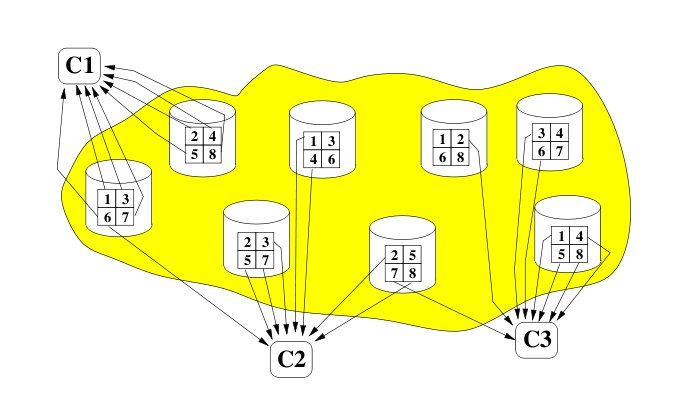
\includegraphics[scale=.4]{replicacao-pura.jpg}
   %         \caption{Sistema com replica��o pura \cite{Plank:2004}}
   %         \label{fig4:srp}
   %     \end{minipage}\hfill
   %     \begin{minipage}[b]{0.48 \linewidth}
   %         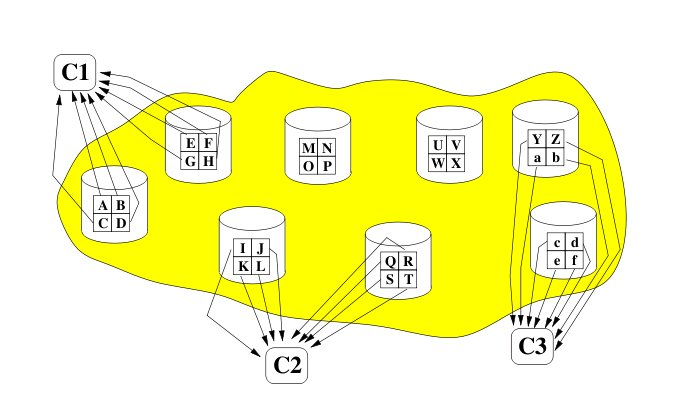
\includegraphics[scale=.4]{codigos-RS.jpg}
   %         \caption{Sistema com c�digos RS \cite{Plank:2004}}
   %         \label{fig5:crs}
   %     \end{minipage}
   % \end{figure}


   \begin{figure}[h]
     \centering
     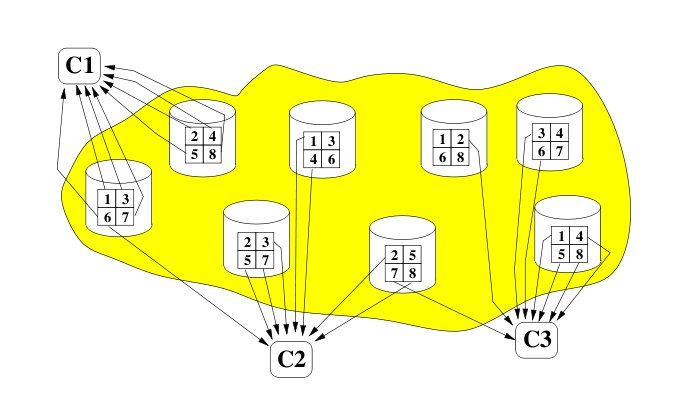
\includegraphics[scale=.6]{replicacao-pura.jpg}
     \caption{Sistema com replica��o pura \cite{Plank:2004}}
     \label{fig4:srp}
   \end{figure}

   \begin{figure}[h]
     \centering
     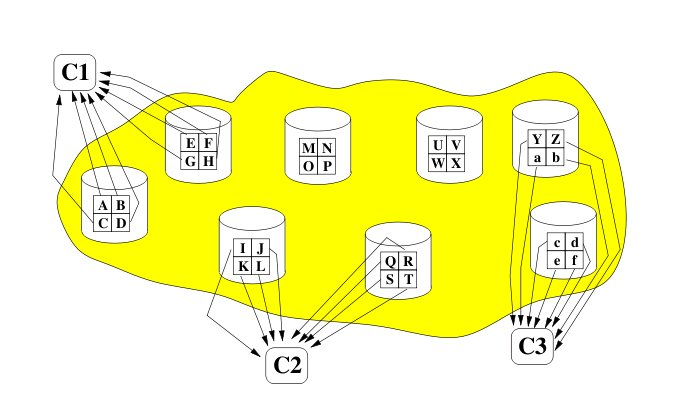
\includegraphics[scale=.6]{codigos-RS.jpg}
     \caption{Sistema com c�digos RS \cite{Plank:2004}}
     \label{fig5:crs}
   \end{figure}


 \section{Hadoop}

Atualmente, o Google � uma empresa de consulta e publicidade e � capaz de fornecer os seus servi�os devido a investimentos em armazenamento distribu�do em larga escala e a capacidade de processamento, estes desenvolvidos \emph{in-house}.

Essa capacidade � fornecida por um grande n�mero de PCs, pelo Google File System (GFS), um sistema de arquivos redundantes em \emph{cluster}, pelo sistema operacional GNU/Linux e pelo MapReduce, um \emph{middleware} de processamento paralelo de dados.

Em 2004, um artigo~\cite{Dean:2004}, que foi publicado por
profissionais da Google, prop�s o MapReduce. Em 2006, estes
profissionais, juntamente com Doug Cutting do Yahoo!, formaram um
sub-projeto do Apache Lucene\footnote{http://www.apache.org} que foi
chamado Hadoop\footnote{http://hadoop.apache.org/}.

Mais recentemente, o projeto Apache Hadoop tem desenvolvido uma
reimplementa��o de partes do GFS e MapReduce e muitos grupos da
comunidade de software livre posteriormente abra�aram essa tecnologia,
permitindo-lhes fazer coisas que eles n�o poderiam fazer em m�quinas
individuais. O Hadoop est� dispon�vel em c�digo fonte sob
licenciamento Apache \emph{license} (compat�vel com GPL).

O Hadoop � um \emph{framework} para executar aplica��es em
armazenamento distribu�do de grande volume de dados que pode ser
constru�do com \emph{commodity hardware}, que � facilmente acess�vel e
dispon�vel.  O Hadoop n�o � um \emph{framework} can�nico. Ele foi
projetado para aplica��es que atualizam dados da seguinte forma: uma
escrita e muitas leituras, atrav�s de acessos por \emph{batch}, com
tamanho da ordem de petabytes, organizados de forma n�o estruturada,
com esquema din�mico e integridade baixa.  Uma lista de aplica��es e
organiza��es que usam o Hadoop pode ser encontrada em
\cite{HadoopWiki:2010}.

Em poucas palavras, o Hadoop disponibiliza um armazenamento
compartilhado (HDFS) e um sistema de an�lise (MapReduce) que comp�em o
seu \emph{kernel}.

\subsection{MapReduce}

O MapReduce utiliza algoritmos de ordena��o para reconstruir sua base de dados.  Um bom uso para o MapReduce s�o aplica��es cujos dados s�o escritos uma vez e lidos muitas vezes. S�o dados n�o estruturados como texto ou imagens. O MapReduce tenta colocar esses dados no n� onde s�o feitas as computa��es, desta forma, o acesso aos dados � r�pido, pois � local \cite{White:2009}.

O MapReduce pode resolver problemas gen�ricos, cujos dados podem ser divididos em matrizes de dados, para cada matriz a mesma computa��o necess�ria (sub-problema) e n�o existe necessidade de comunica��o entre as tarefas (sub-problemas). A execu��o de um t�pico \emph{job} do MapReduce pode ser assim descrita:

\begin{itemize}
    \item Itera��o sobre um n�mero grande de registros
    \item Map extrai algo de cada registro (chave, valor)
    \item Rearranjo (\emph{shuffle}) e ordena��o de resultados intermedi�rios por (chave, valor)
    \item Reduce agrega os resultados intermedi�rios
    \item Gera��o da sa�da
\end{itemize}

Um programas para execu��o no HFS/MapReduce que podem ser escritos em v�rias linguagens como Java, Ruby, Python e C++.


\subsection{Arquitetura do Hadoop \emph{Distributed File System}}

Um \emph{cluster} do HDFS � composto por um �nico NameNode, um
servidor-mestre que gerencia o sistema de arquivos e controla o acesso
aos arquivos de clientes. H� uma s�rie de DataNodes, geralmente um por
n� do \emph{cluster}, que gerenciam o armazenamento anexado ao n� em
que s�o executados. A Figura~\ref{fig6:hfs} mostra o NameNode e os
DataNodes.

Uma t�pica arquitetura de rede em dois n�veis para um \emph{cluster}
Hadoop � constru�da por v�rios \emph{racks} interligados por um
comutador como mostra a Figura~\ref{fig5:hc}. Cada \emph{rack} por sua
vez � formado por v�rios n�s (m�quinas) e seus discos, estes tamb�m
interligados por um comutador.

    \begin{figure}[h]
      \centering
      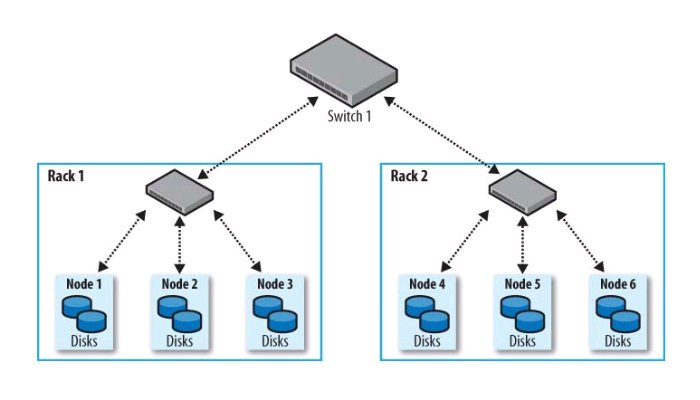
\includegraphics[scale=0.6]{hadoop-cluster.jpg}
      \caption{Arquitetura de rede em dois n�veis para um cluster Hadoop~\cite{Hadoop:2010}}
      \label{fig5:hc}
    \end{figure} 

O NameNode executa opera��es no sistema de arquivos, como \emph{open}, \emph{close}, \emph{rename} de arquivos e de diret�rios.

HDFS disponibiliza espa�o para sistema de arquivos e permite que os
dados do usu�rio sejam armazenados em arquivos. Internamente, um
arquivo � dividido em um ou mais blocos e esses blocos s�o armazenados
em um conjunto de DataNodes. A Figura~\ref{fig7:hfs} mostra DataNodes
e seus blocos. O tamanho \emph{default} de cada bloco � 64MB.

    \begin{figure}[htbp]
      \centering
      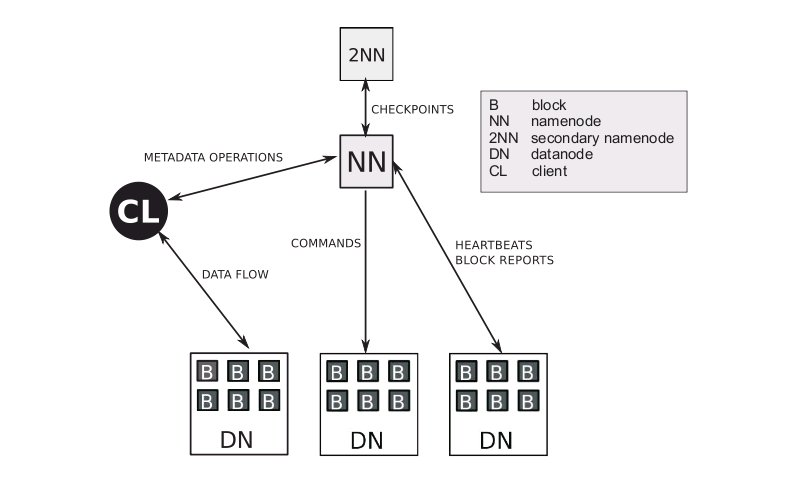
\includegraphics[scale=.6]{HDFS-arquitetura-2.jpg}
      \caption{Arquitetura do HDFS \cite{TR-IC-10-24}}
      \label{fig6:hfs}
    \end{figure} 

Os DataNodes respondem aos pedidos de leitura e escrita de clientes do
sistema de arquivos e tamb�m executam a cria��o, elimina��o e
replica��o de blocos sob instru��o do NameNode. O n�mero de r�plicas �
geralmente 3. A 1$^a$ r�plica fica local, no mesmo n� do c�digo do
cliente. A 2$^a$ r�plica fica em um n� em outro \emph{rack} e a 3$^a$
r�plica fica nesse �ltimo \emph{rack} em outro n�. As 2$^a$ e 3$^a$
r�plicas n�o s�o locais ao bloco replicado.

O NameNode e DataNode s�o partes do \emph{software} projetado para
rodar em \emph{commodity hardware}. Essas m�quinas normalmente
executam um sistema operacional GNU/Linux.

HDFS � constru�do usando a linguagem Java. Qualquer m�quina que suporte
Java pode executar o NameNode ou o DataNode \cite{Hadoop:2010}.

\begin{figure}[h]
  \centering
  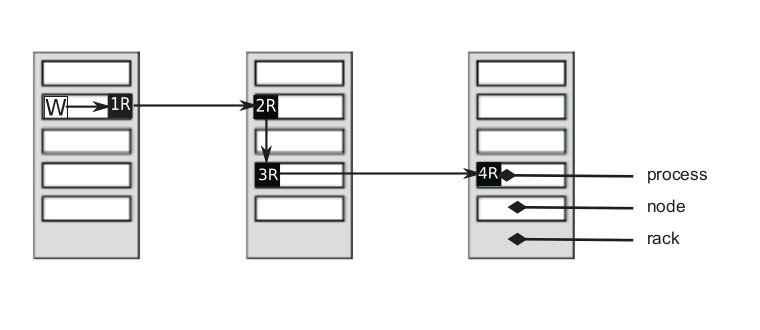
\includegraphics[scale=.5]{HDFS-arquitetura-replicacao-2.jpg}
  \caption{Arquitetura do HFS - Datanodes e Blocos \cite{White:2009}}
  \label{fig7:hfs}
\end{figure} 

Os protocolos do HDFS usam o protocolo TCP/IP. O cliente fala o
protocolo ClientProtocol com o NameNode atrav�s de uma porta. Os
DataNodes falam o protocolo DataNodeProtocol com o NameNode. Esses
protocolos executam uma \emph{Remote Procedure Call} (RPC). O NameNode
n�o inicia chamadas RPCs. Ele responde a chamadas RPCs feitas pelo
DataNodes e pelos clientes.


\subsection{Codifica��o por apagamento}

Existe uma nova caracter�stica proposta em 2009 para implementa��o de
uma camada de codifica��o por apagamento no Hadoop utilizando
RAID~\cite{HDFS-503:2010} e uma mais recente utilizando c�digos
RS~\cite{MR-1969:2010}.

A vers�o atual do Hadoop utiliza apenas a t�cnica de replica��o
\cite{White:2009} para obter disponibilidade e confiabilidade de
dados. A inclus�o da codifica��o por apagamento ser� feita com o
objetivo de reduzir o tamanho do armazenamento do HDFS.


 \section{Proposta}

\subsection{Objetivos}

Esta proposta apresentar� uma an�lise da viabilidade da implementa��o
pr�tica de v�rias t�cnicas de codifica��o por apagamento no HDFS, as
altera��es no Hadoop e a efic�cia dessas altera��es. Esta proposta �
uma contribui��o para \emph{software} livre em sistemas distribu�dos.

O objetivo do uso da codifica��o � reduzir o tamanho do armazenamento
utilizando para isso a redu��o do fator de replica��o de um bloco e
codifica��o de um conjunto de blocos (a partir de um bloco inicial) de
tal modo que a probabilidade de falha de um bloco permane�a a mesma
que antes ou diminua.

Os testes ser�o feitos para mostrar a efic�cia das altera��es no HDFS:
quanto de espa�o em disco foi economizado e o tempo de lat�ncia de
leitura de arquivos. Tamb�m est� prevista a implementa��o e valida��o
em software dos algoritmos RS e Tornado, que possibilitar� a valida��o
da funcionalidade desses algoritmos.

\subsection{M�todos}

Este trabalho ir� estender e alterar c�digo fonte distribu�do sob a
licen�a Apache. Espera-se a intera��o e colabora��o com os
desenvolvedores. Atualmente, Rodrigo Malta Schimdt, ex-aluno do
Instituto de Computa��o da Unicamp e um dos respons�veis pela inclus�o
de t�cnicas de codifica��o por apagamento no HDFS tem contribu�do com
v�rias ideias para a realiza��o deste trabalho.

Os testes poder�o utilizar:

\begin{itemize}
\item m�quinas do Instituto de Computa��o da Unicamp, principalmente
  do LSD (Laborat�rio de Sistemas Distribu�dos);
\item m�quinas do ambiente computacional do CENAPAD-SP (Centro
  Nacional de Processamento de Alto Desempenho em S�o Paulo)
\item a nuvem do AWS (Amazon \emph{Web Services}).
\end{itemize}

Na tabela~\ref{tab2:ccr} o Modelo 1 � modelo atual do HDFS, o Modelo 2
� modelo em implementa��o com caracter�stica HDFS-503
\cite{HDFS-503:2010} e as Propostas 3, 4 e 5 s�o propostas de
implementa��o de algoritmos de codifica��o para este trabalho. A
disponibilidade, a probabilidade de corrup��o de um arquivo e o espa�o
de armazenamento foram adaptadas de \cite{MR-1969:2010} e de
\cite{Bhagwan:2003}. A possibilidade de falhas nas m�quinas est�o
atreladas a uma boa escolha da distribui��o dos blocos pelos
dispositivos de armazenamento.

\begin{table}

{\small

\singlespacing

  \begin{center}
    \begin{tabular}{|p{2.0cm}||p{3cm}||p{3cm}||p{2.5cm}||p{2.0cm}|} \hline

Proposta/ Modelo & Codifica��o\phantom{\Large X} & Disponibilidade & Probabilidade de corrup��o de um arquivo & Espa�o de armazenamento \\ \hline

1\phantom{\Large X}  & sem codifica��o, fator replica��o = $n$ & baixa em rela��o ao espa�o de armazenamento & $O(p^n)$ & $nx$ \\[2pt] \hline

2\phantom{\Large X}  & C�digos RAID, 1 bloco de paridade, stripe = 10 blocos, fator replica��o = 2 & permite falha em 1 m�quina  & $O(p^4)$ & $2.2x$ \\ \hline

3\phantom{\Large X} & C�digos RS RAID, 4 blocos de paridade, stripe = 10 blocos, fator replica��o = 1 & permite falha em 3 m�quinas & $O(p^5)$ & $1.4x$ \\ \hline

4\phantom{\Large X} & C�digos RS, 4 blocos de paridade, fator replica��o = 1, com $n$ m�quinas & permite falha em at� $(3m + 1)$ m�quinas & $\Omega(p^{3m+2})$ & at� $5x$ \\ \hline

5\phantom{\Large X} & C�digos Tornado, 4 blocos de paridade, fator replica��o = 1, com $n$ m�quinas & permite falha em at� $(3m + 1)$ m�quinas & $\Omega(p^{3m+2})$ & at� $5x$ \\ \hline

    \end{tabular}
\caption{Compara��o entre algoritmos de codifica��o por apagamento e replica��o}
\label{tab2:ccr}
  \end{center}

em que:\\
%$O$ e $\Omega$: nota��o assint�tica, significando \emph{upper bound} e \emph{lower bound} respectivamente\\
$p$ = probabilidade de perda do bloco, $0 < p < 1$\\
$x$ = tamanho do armazenamento em disco de um bloco\\
$m$ = n�mero de fragmentos do bloco inicial antes da codifica��o\\
$n = 4m$ � n�mero de blocos codificados a partir a um bloco inicial; o bloco codificado $b_{i}$ est� armazenado na m�quina $d_{i}$, para $1 \leq i \leq m$; o bloco inicial e a primeira r�plica est�o na m�quina $d1$\\
}

\end{table}

\subsection{Forma de An�lise dos Resultados}

N�s poderemos utilizar alguns \emph{ebooks} do Projeto Gutenberg e do
Portal Dom�nio P�blico como entrada de dados de alguns dos testes:

\begin{itemize}
   
\item {Teste de funcionalidade dos algoritmos de codifica��o e de
    decodifica��o RS e de outra codifica��o como Tornado}

     % com dois PCs interconectados (via porta serial, padr�o RS-232 ou
     % via porta USB), sob sistema operacional GNU/Linux e e representar
     % o que acontece de algum modo: arquivo de log, anima��o.

   \item {Teste \emph{cluster} Hadoop  0.21.0} que utiliza apenas replica��o

   \item {Teste \emph{cluster} Hadoop 0.21.0 com caracter�stica
       HDFS-503} que utiliza replica��o e codifica��o por apagamento
     \cite{HDFS-503:2010}

\end{itemize}

% Este \emph{patch} pretende implementar uma camada opcional de
% codifica��o por apagamento sob o HDFS. O objetivo deste \emph{patch} �
% reduzir o volume de armazenamento do HDFS.

% � poss�vel que sejam usados entrada de dados como imagens, desde que
% possam ser disponibilizadas nas m�quinas utilizadas nos testes: dados
% dos laborat�rios do IC-Unicamp e da Embrapa.

Estamos prevendo duas fases de teste:

\begin{description}

   \item [testes de funcionalidade e de inje��o de falhas] testar os algoritmos que criam  os blocos codificados (dados e paridade) e os mant�m; testar os algoritmos que atendem os pedidos de leitura (r�plica); testar os algoritmos que percebem r�plicas indispon�veis e as reconstroem a partir dos blocos codificados (para isso utilizar possivelmente o Zookeeper, um servi�o de coordena��o de processos de aplica��es em sistemas distribu�dos); testar os algoritmos que percebem blocos indispon�veis e reconstroem as r�plicas (se indispon�veis); esta fase ser� executada em ambiente virtualizado;

   \item [testes de desempenho, de tamanho do armazenamento e de inje��o de falhas] obter uma aproxima��o do tamanho do armazenamento (dados e paridade) para conjuntos de arquivos que ocupem espa�o original do tamanho de alguns gigabytes e terabytes; esta fase ser� executada em ambiente o mais real poss�vel.

\end{description}

Os algoritmos de codifica��o e de decodifica��o poder�o permitir parametrizar:

\begin{itemize}

   \item n�mero de peda�os que o bloco original � dividido antes da gera��o dos blocos codificados
   \item n�mero de blocos de paridade (redund�ncia)
   \item fator de replica��o
%\footnote{Este par�metro � atualmente configurado no HFS como dfs.replication.}
\end{itemize}

{\tiny
\begin{enumerate}
\item Cr�ditos do mestrado
\item Exame de qualifica��o do mestrado
\item Revis�o bibliogr�fica
\item Implementa��o
\item Realiza��o de testes
\item Escrita da disserta��o de mestrado
\item Prepara��o de artigo para congresso ou revista
\item Defesa da disserta��o
\end{enumerate}

\begin{center}
\begin{tabular}{|l||c|c|c|c|c||c|c|c|c|c|c|c|}
\hline
&\multicolumn{5}{l||}{2010}&\multicolumn{6}{l|}{2011}&\multicolumn{1}{l|}{2012}\\
\cline{2-13}
Atividade & 3--4 & 5--6 & 7--8 & 9--10 & 11--12 & 1--2 & 3--4 & 5--6 & 7--8 & 9--10 & 11--12 
& 1--2 \\ \hline
\hline\hline
1 & o&  o&  o&  o&  o&   &   &   &   &   &   &  \\ \hline
2 &  &   &   &  o&   &   &   &   &   &   &   &  \\ \hline
3 & o& oo& oo& oo& oo& oo& oo&  o&  o&  o&  o&  \\ \hline
4 &  &   &  o& oo& oo& oo& oo& oo& oo& oo& oo&  \\ \hline
5 &  &  o&  o& oo& oo& oo& oo& oo& oo& oo& oo&  \\ \hline
6 &  & oo& oo& oo& oo& oo&  o&  o&  o&  o&  o&  \\ \hline
7 &  &   &   &   &   &   &   &  o&  o&  o&   &  \\ \hline
8 &  &   &   &   &   &   &   &   &   &   &   &  o\\ \hline
\hline
\end{tabular}
\end{center}
}


% \subsection{Vantagens e Limita��es deste trabalho}

% O modelo estudado neste trabalho envolve canal bin�rio, sim�trico e sem mem�ria.

% Segundo \cite{Woitaszek:2007}, para sistemas de armazenamento, a codifica��o por apagamento baseada em opera��es simples, tais como XOR RAID e c�digos Tornado, s�o prefer�veis. Apesar de que um mecanismo externo deva ser utilizado para detectar erros, as opera��es de XOR podem ser realizadas rapidamente e resultar em alto \emph{throughput} das opera��es de codifica��o e decodifica��o.

% As codifica��es de blocos que ser�o estudadas e implementadas s�o: c�digos Reed-Solomon (modelo 3 e proposta 4) e c�digos Tornado (proposta 5). S�o algoritmos muito estudados e com conhecidas implementa��es.

\subsection{Contribui��es deste trabalho}

\subsubsection*{\emph{Overview} de Codifica��o por Apagamento}

A revis�o bibliogr�fica desse tema tem exigido tempo e dedica��o, devido a exist�ncia de poucas pesquisas experimentais publicadas sobre o tema. Uma dificuldade encontrada por quem estuda codifica��o por apagamento � que n�o existe uma nomenclatura unificada \cite{Plank:2009}. Tamb�m segundo \cite{CS540:2010}, existem poucos pesquisadores que s�o programadores de sistemas e que fazem propostas neste tema.

% Uma classifica��o para c�digos de blocos pode ser encontrada na figura~\ref{fig4:cbc}.

%    \begin{figure}[h]
%      \centering
%      \includegraphics[scale=1]{blockcodes.png}
%      \caption{Uma classifica��o para c�digos de blocos \cite{MathWorks:2010}}
%      \label{fig4:cbc}
%    \end{figure} 

Uma classifica��o para c�digos de blocos pode ser encontrada em \cite{MathWorks:2010}.

\subsubsection{Submeter as altera��es e sugest�es como contribui��o ao Hadoop}

As altera��es e sugest�es para uso das codifica��es por apagamento no
Hadoop ser�o propostas a comunidade por meio do site da Apache
\emph{Software Foundation}, como foi proposta a vers�o inicial de
codifica��o por apagamento no HDFS~\cite{HDFS-503:2010} e a segunda
vers�o com c�digos Reed-Solomon~\cite{MR-1969:2010}.



\section{Refer�ncias Bibliogr�ficas}

\begin{frame}[allowframebreaks,allowdisplaybreaks]{Refer�ncias Bibliogr�ficas}

%  \smaller[5]

  \bibliographystyle{plain}
%  \setbeamertemplate{bibliography item}[book] 
  \bibliography{apresentacao}

\end{frame}



\end{document}
